\documentclass[border=4pt]{standalone}
\usepackage{tikz}
\usetikzlibrary{arrows}
\begin{document}
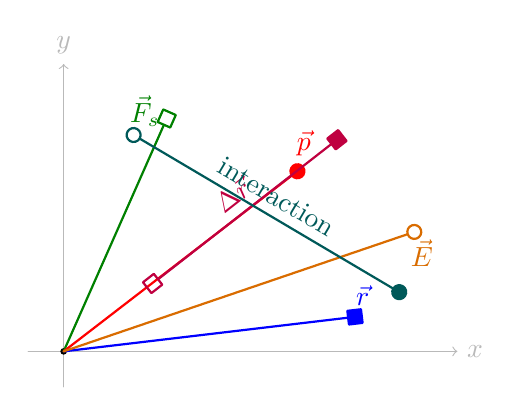
\begin{tikzpicture}[line cap=round]
  \draw[gray!55,->] (-.45,0) -- (5,0) node[right]{$x$};
  \draw[gray!55,->] (0,-.45) -- (0,3.65) node[above]{$y$};
  \fill (0,0) circle (1.2pt);

  \draw[blue,line width=.8pt,-square] (0,0) -- (3.8,.45) node[above]{$\vec r$};
  \draw[green!50!black,line width=.8pt,-{open square}] (0,0) -- (1.35,3.05) node[left]{$\vec F_s$};
  \draw[red,line width=.8pt,-*] (0,0) -- (3.05,2.35) node[above,sloped]{$\vec p$};
  \draw[orange!85!black,line width=.8pt,-o] (0,0) -- (4.55,1.55) node[below,sloped]{$\vec E$};
  \draw[purple,line width=.8pt,{open square}-{square}] (1.05,.8) -- (3.55,2.75) node[midway,above,sloped]{$\Delta\vec r$};
  \draw[teal!70!black,line width=.8pt,{o}-{*}] (.8,2.8) -- (4.35,.7) node[midway,above,sloped]{interaction};
\end{tikzpicture}
\end{document}
